\chapter{Algorithmic Strategies}
\label{cha:partition_strategy}

In the last chapter we described how the CellDivider tool interacted with the routing framework and the already existing data structures. However, probably the most interesting part is what CellDivider does in order to achieve routing big and complex cells using the divide-and-conquer scheme. \\

As exposed in Section \ref{sec:routing}, two approaches for divide-and-conquer can be considered: bottom-up and top-down. The last one would imply to first create some general routing connections and then work at a lower level, whereas the first one implies first routing little zones and then expand the routing to bigger ones, such as an entire cell. In this project, the bottom-up methodology seems the most natural approach. A top-down scheme would imply first routing the connections of parts far away in the cell, which would potentially occupy spaces needed for the detailed local routing. Given the characteristics of the tool, a bottom-up approach seems a more easily implementable option. The idea would be to solve parts of a given cell so that finally the whole routing problem becomes simpler than it originally was.  \\

The remainder of the chapter is structured in two sections. Section \ref{sec:partitionalgorithms} exposes several methods that can be used to route a part of a cell. Section \ref{sec:metaalgorithms} explains how to use such partial routings in order to find a valid solution for the whole cell.

\section{Partition algorithms}
\label{sec:partitionalgorithms}

A partition algorithm decides how to partially route some part of a cell. As explained before, the most basic approach would be to absolutely ignore what lies on the other sides of the limits when doing a partial routing. This is dangerous because, as stated before, a bad partial solution could lead the global problem to be unsatisfiable. For example, consider routing the cell in Figure \ref{fig:2bandesbuida} by first routing the left half. Figure \ref{fig:2bandesmitja} shows what the partition would look like and a possible solution the that partial problem. Note that, on column 4, all horizontal positions are occupied. This is entirely valid on the partial solution as the green node does not need to be connected to any component on the right side. But when the partial solution is incorporated to the total cell and we try to route it, we are unable to find a valid routing because the green net cannot be connected as shown in Figure \ref{fig:2bandesplena}. \\

\begin{figure}[h!]
  \centering
  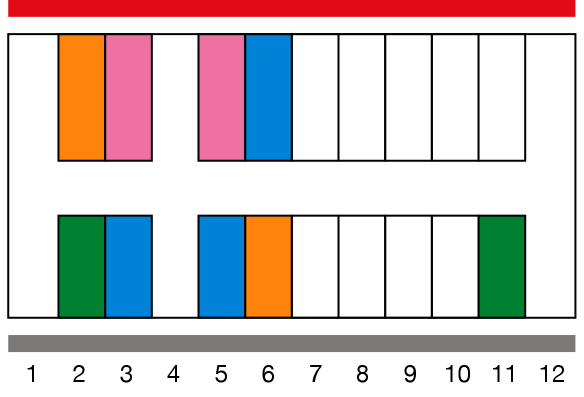
\includegraphics[scale=0.5]{img/design/2bandesbuida.png}
  \caption{Input for CellDivider}
  \label{fig:2bandesbuida}
\end{figure} 

\begin{figure}[h!]
  \centering
  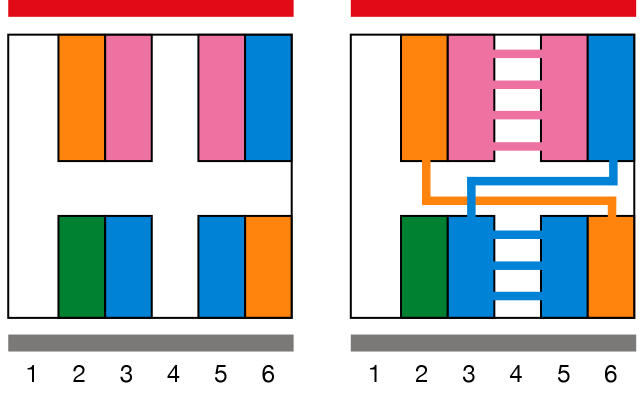
\includegraphics[scale=0.5]{img/design/2bandesmitja.png}
  \caption{Partial problem and solution}
  \label{fig:2bandesmitja}
\end{figure} 

\begin{figure}[h!]
  \centering
  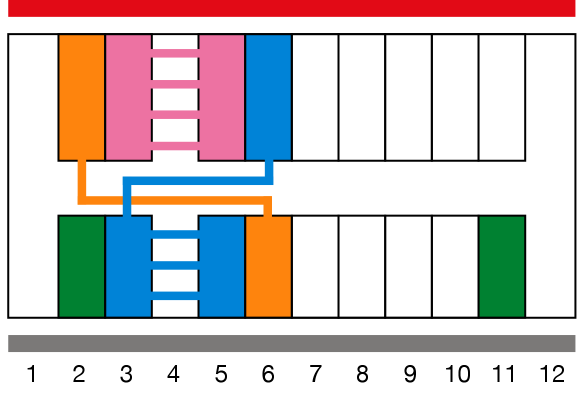
\includegraphics[scale=0.5]{img/design/2bandesplena.png}
  \caption{Final routing problem}
  \label{fig:2bandesplena}
\end{figure} 

This example perfectly illustrates the situation of a partial routing turning the whole cell unroutable. It must be kept in mind that when CellRouter returns a satisfying model it will probably not be optimal, so high-congested zones may appear. It is also important to notice that the design rules may be very strict, so finding a situation where a partial solution renders the whole problem unsatisfiable has proved to be quite usual. To cope with this problem, the following partitioning approaches try to keep some information on what lies on the parts of the cell that are not being routed in the partial problem.

\subsection{Realistic Partitioning}

Consider a more general form of routing a part of the cell, where we want to solve the routing problem from column $n$ to column $m$. The realistic partitioning algorithm considers the central part of the cell, from columns $n$ to $m$, and certain regions at their right and left. The main idea is that any signal which has a terminal on the central zone and another one on any of the side zones should be granted an exit to the terminal outside the central zone. Additionally, if a signal has a terminal in the right and left zone but none in the central zone, it should be imposed that a path crossing the central zone exists. \\

The left zone ranges from column $ini$ to column $n$, whereas the right zone ranges from column $m$ to $end$. $ini$ is the leftmost column where there is a terminal that must be connected to another terminal on either the central or right zone. $end$ is defined the other way around. A temporal cell is created, where the width is $end - ini$. The zone from $n$ to $m$ receives an exact copy of the original cell from $n$ to $m$. The zone from $ini$ to $n$ and from $m$ to $end$, however, will only contain the closer terminals to $n$ and $m$ such that they are required to be connected with the central zone or the opposite side. Finally, the positions where the connection pins are considered valid are calculated and the cell can be routed. After the cell is routed, all wires that are not part of a subnet when the solution is copied on the original cell are removed. The function looks as follows. \\

\small
\begin{algorithmic}
\Function{Realistic partitioning}{$G$ grid, $n$ and $m$ column indexes} \\
\State Find signals in the center, left and right
\State $ini \gets 0$
\State $end \gets G$'s width
\State $partial\_signals \gets \{\}$
\State $partial\_terminals \gets \{\}$
\ForAll{signal in $G$} 
	\If {signal in left and in either center or right, or viceversa}
		\State Save closer signal appearance to $n$ and $m$
		\State Update $ini$ and $end$ accordingly
	\EndIf
	\If {signal will be in the partial cell}
		\State Add signal into $partial\_signals$
		\State Add wether it needs an external pin or not into $partial\_terminals$
	\EndIf
\EndFor \\

\State $partial\_pins \gets \{\}$
\ForAll{$pin$ in $G$} 
	\If {$pin$'s column index betweem $ini$ and $end$}
		\State Add $pin$ to $partial\_pins$ substracting $ini$ to column index
	\EndIf
\EndFor \\

\State $R \gets$ new grid with width $end - ini$ 
\State Add $partial\_signals$, $partial\_terminals$ and $partial_pins$ to $R$ \\

\ForAll{$element$ (vertex or edge) in $R$}
	\State $original \gets$ mapping of $element$ in $G$ 
	\If {$original$ column between $n$ and $m$} 
		\State $element \gets $ signal of $original$ in $G$
	\ElsIf{$element$ on lowest level}
		\State $element \gets locked\_signal$ 
	\Else
		\State $element \gets free\_signal$
	\EndIf
\EndFor \\

\ForAll{$terminal$ needed outside $n$-$m$ range}
	\State Add $terminal$ to $R$
\EndFor \\

\State Save $R$ to a file
\State Call CellRouter over $R$
\If {call is unsat}
		\State \Return $unsat$
\EndIf
\State Load solved $R$ from file \\

\ForAll{$element$ (vertex or edge) in $R$}
	\State $original \gets$ mapping of $element$ in $G$ 
	\If {$original$ column between $n$ and $m$} 
		\State $original \gets $ signal of $element$ in $R$
	\EndIf
\EndFor
\State Clean $G$ grid  
\State \Return $routing\_time$ \\
\EndFunction
\end{algorithmic} 
\normalsize

For example, we want to route the zone defined by $n$ and $m$ on the cell in Figure \ref{fig:RealDivBuida}. We need to ensure that both signals on column 6 have an exit to the other parts of the cell where they are required, which are columns 3 and 9. Additionally, on these two columns there is a terminal of the same signal that should cross the central zone. We need to set $ini$ to column 3 and $end$ to column 9. Now, as explained earlier, the zone between $n$ and $m$ will have all the terminals included and the rest of the partial cell will only have the required terminals, as shown in Figure \ref{fig:RealDivParcial}. \\

\vspace{10 mm}
\begin{figure}[h!]
  \centering
  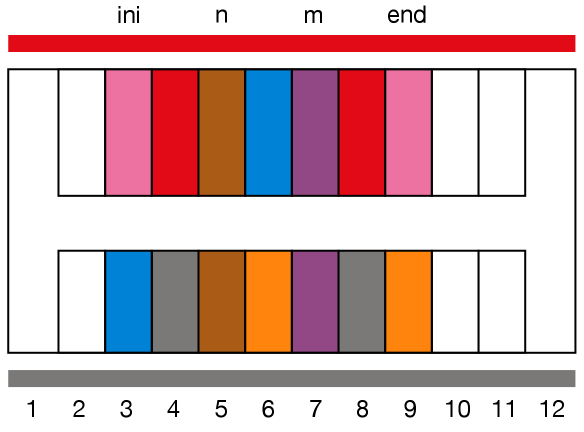
\includegraphics[scale=0.5]{img/design/RealDivBuida.png}
  \caption{Input for CellDivider}
  \label{fig:RealDivBuida}
\end{figure} 

\begin{figure}[h!]
  \centering
  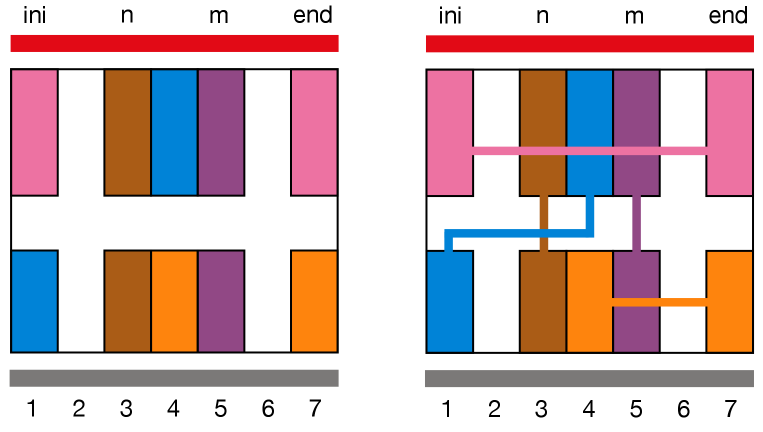
\includegraphics[scale=0.5]{img/design/RealDivMitja.png}
  \caption{Partial problem and solution}
  \label{fig:RealDivParcial}
\end{figure} 


After the partial routing is completed, only the signals routed in the range from column $n$ to column $m$ are copied back to the original cell. All the wires that are not in a path between two terminals of the central zone are also removed. This would be the case of a wire that simply crossed the central region but did not have any terminal in it. Since we only wanted to impose that such a path existed, the routing tool will occupy again those positions if needed. Figure \ref{fig:RealDivFinal} shows how the final cell looks like after the partial solution has been added. Notice that all wires that did not begin and end in the central zone have disappeared, but the path they occupied is available. \\


\begin{figure}[h!]
  \centering
  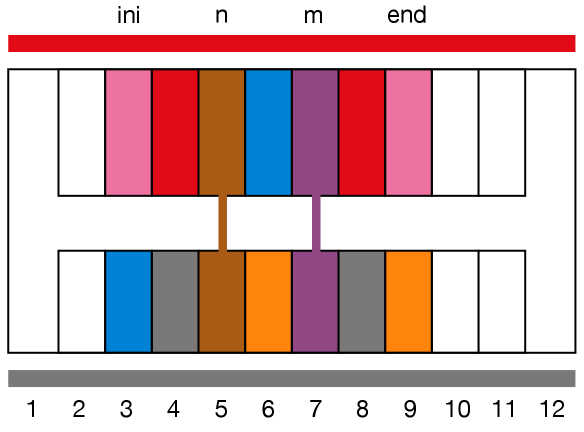
\includegraphics[scale=0.5]{img/design/RealDivFinal.png}
  \caption{Final routing problem}
  \label{fig:RealDivFinal}
\end{figure} 


Now let's take the example that was shown before, where a cell was rendered unsatisfiable. If the partial routing is done using realistic partitioning, Figure \ref{fig:realmitja} shows how the partial routing problem and solution looks like. Given that there is a signal in column 2 whose closer terminal is in column 11 on the original cell, the partial cell will have to include up until that column. However, since it is the only signal shared between the $n$-$m$ zone and the rest of the cell, it will be the only terminal from column 6 to column 10 in the partial cell. Finally, Figure \ref{fig:realfinal} shows the final routing problem. Notice that now a path for the signal that before rendered the cell unsatisfiable exists. This does not guarantee that now the total cell will have a valid routing, but chances are higher than before. \\

\begin{figure}[h!]
  \centering
  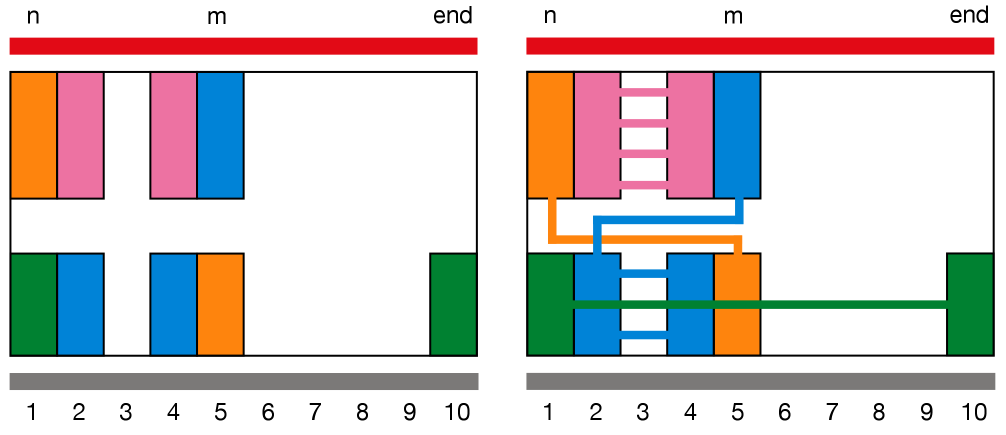
\includegraphics[scale=0.5]{img/design/RealMitja.png}
  \caption{Partial problem and solution}
  \label{fig:realmitja}
\end{figure} 

\begin{figure}[h!]
  \centering
  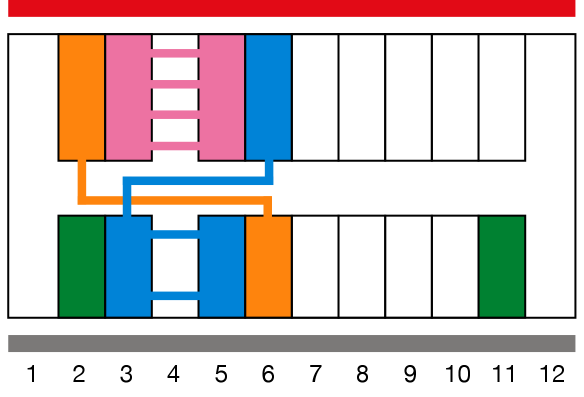
\includegraphics[scale=0.5]{img/design/RealFinal.png}
  \caption{Final routing problem}
  \label{fig:realfinal}
\end{figure} 

Notice that a number of variations exist for this partitioning algorithm. For instance, when copying the partial solution to the original cell, all wires from $n$ to $m$ can be copied, not only the ones beginning and ending in that range. Another option would be copying all the wires of the partial solution, regardless of what zone they are in. Another option would be, when preparing the partial cell, including all terminals outside the central zone and not only those strictly required to be routed. It is specially useful when multiple partial routings are performed on a single cell, given that zones that might look empty for a partial solution could have already been occupied by an earlier routing.  \\

\subsection{Boundary-Conscious Partitioning}

This partitioning approach is similar to the one described in the previous subsection. Once again we intend to route a cell from column $n$ to a column $m$. However, the idea is to approximate all terminals outside the routing zone that should be connected with signals that are between the $n$-th and $m$-th columns or that should simply cross that zone. \\

Consider the case of the right part of the zone we want to route. The algorithm will find, for every signal that is both in the right part and outside it, the terminal that is closer to the boundary between the zones. The partial cell can be created when the number of signals to approximate in both sides is known. As in the realistic partitioning approach, the zone between $n$ and $m$ is entirely copied. As for the other parts, respecting the closeness of every terminal to the boundary, fake terminals are added to represent that they must be connected with a terminal in that zone. The pseudocode, which is very similar to the one in previous subsection, is as follows. \\

\small
\begin{algorithmic}
\Function{Boundary-Conscious Partitioning}{$G$ grid, $n$ and $m$ column indexes} \\
\State Find signals in the center, left and right
\State $partial\_signals \gets \{\}$
\State $partial\_terminals \gets \{\}$
\ForAll{signal in $G$} 
	\If {signal in left and in either center or right, or viceversa}
		\State Save closer signal appearance to $n$ and $m$
		\State Decide if placing the terminal on $p$ or $n$ zone if needed
	\EndIf
	\If {signal will be in the partial cell}
		\State Add signal into $partial\_signals$
		\State Add wether it needs an external pin or not into $partial\_terminals$
	\EndIf
\EndFor 
\State Calculate how many terminals will be added at left and right
\State $partial_width \gets m - n + termianls_left + terminals_rigth$ \\

\State $partial\_pins \gets \{\}$
\ForAll{$pin$ in $G$} 
	\If {$pin$'s column index betweem $ini$ and $end$}
		\State Add $pin$ to $partial\_pins$ substracting $ini$ to column index
	\EndIf
\EndFor \\

\State $R \gets$ new grid with width $partial_width$ 
\State Add $partial\_signals$, $partial\_terminals$ and $partial_pins$ to $R$ \\

\ForAll{$element$ (vertex or edge) in $R$}
	\State $original \gets$ mapping of $element$ in $G$ 
	\If {$original$ column between $n$ and $m$} 
		\State $element \gets $ signal of $original$ in $G$
	\ElsIf{$element$ on lowest level}
		\State $element \gets locked\_signal$ 
	\Else
		\State $element \gets free\_signal$
	\EndIf
\EndFor \\

\ForAll{$terminal$ needed outside $n$-$m$ range}
	\State Add $terminal$ to $R$
\EndFor \\

\State Save $R$ to a file
\State Call CellRouter over $R$
\If {call is unsat}
		\State \Return $unsat$
\EndIf
\State Load solved $R$ from file \\

\ForAll{$element$ (vertex or edge) in $R$}
	\State $original \gets$ mapping of $element$ in $G$ 
	\If {$original$ column between $n$ and $m$} 
		\State $original \gets $ signal of $element$ in $R$
	\EndIf
\EndFor
\State Clean $G$ grid  
\State \Return $routing\_time$ \\
\EndFunction
\end{algorithmic} 
\normalsize

The following example illustrates how boundary-conscious partitioning works. Figure \ref{fig:Padbuida} shows the cell we want to route. We decide to partially route the cell between $n$ and $m$. The signal on the top part of column 6 must be connected to the one on the top part of column 3 and both parts of column 10. In the partial problem, we approximate those terminals to the boundary of the zone we want to route. On the left part, the signals on columns 2 and 3 will approach column 4. On the right part we will proceed respecting which signal is closer to the $m$-th column. First comes the signal in column 8, which is already close to the boundary. Following come the terminals on column 10. However, two of them exist at the same distance. In this case, we consider only one of them, the one in the zone which has a lower number of approximated terminals - which is the top zone in this case. Finally, the terminal in column 11 also moves. The partial problem and a possible solution are shown in Figure \ref{fig:Padmitja}. \\

\begin{figure}[h!]
  \centering
  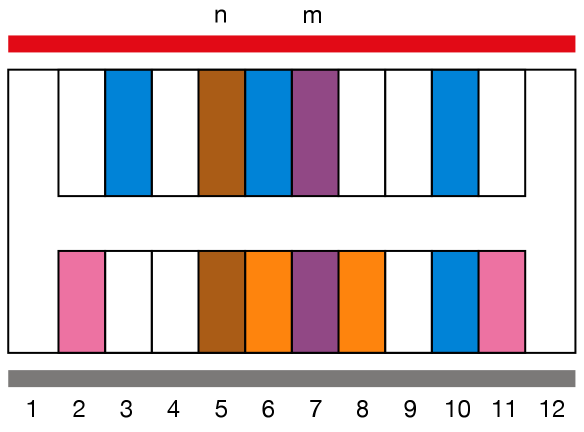
\includegraphics[scale=0.5]{img/design/Padbuida.png}
  \caption{Input for CellDivider}
  \label{fig:Padbuida}
\end{figure} 

\begin{figure}[h!]
  \centering
  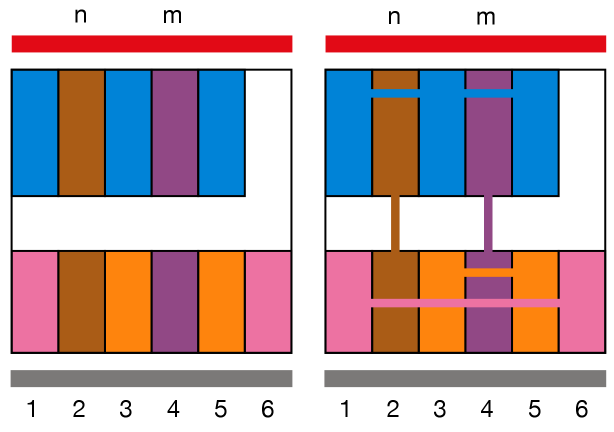
\includegraphics[scale=0.5]{img/design/Padmitja.png}
  \caption{Partial Problem and Solution}
  \label{fig:Padmitja}
\end{figure} 

Figure \ref{fig:Padfinal} shows how the final routing problem looks like once the partial solution is copied. Notice that, since this method alters the geometry of the original problem even more than when using realistic partitioning, all the wires routed outside the $n$-$m$ range need to be discarded. Only wires that both end and begin in between the $n$-th and $m$-th column are kept. \\

\begin{figure}[h!]
  \centering
  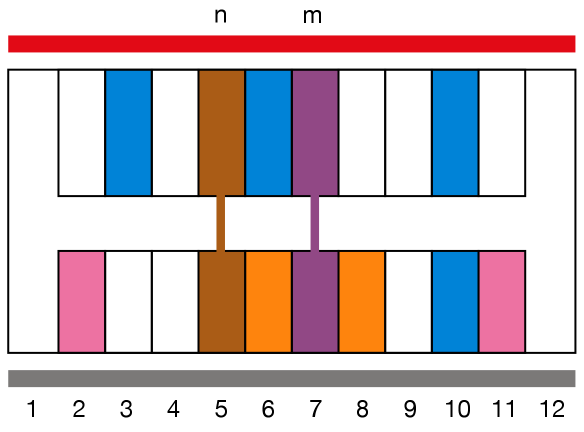
\includegraphics[scale=0.5]{img/design/Padfinal.png}
  \caption{Final routing problem}
  \label{fig:Padfinal}
\end{figure} 


Boundary-conscious partitioning is useful when we are partially routing big cells that have signals which are potentially far away. We can come back to our example in Figure \ref{fig:2bandesbuida}. As we saw in Figure \ref{fig:realmitja}, a lot of empty columns were added in the partial solution. Using boundary-conscious partitioning, all that empty zone can be spared as shown in Figure \ref{fig:Padalt}. The result when copying the information back to the originall cell is the same as the one shown in Figure \ref{fig:realfinal}. Avoiding all that white cell space simplifies the boolean formula, thus reducing the amount of memory and computation time that SAT will need to obtain a partial solution. \\

\begin{figure}[h!]
  \centering
  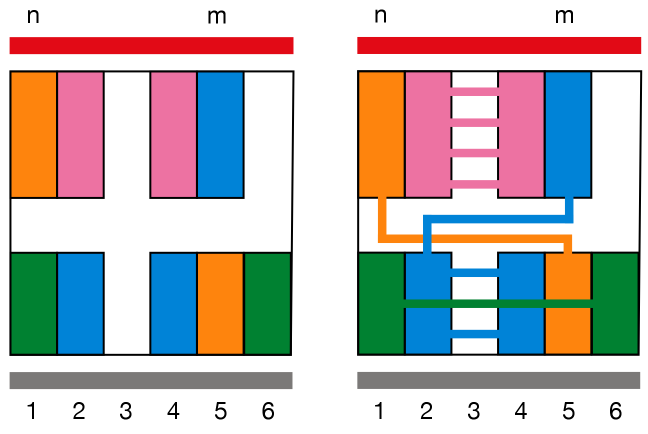
\includegraphics[scale=0.5]{img/design/Padalt.png}
  \caption{Partial problem and solution}
  \label{fig:Padalt}
\end{figure} 

As in the case of realistic partitioning, many variations exist. For example, we could decide to add terminals in both the high and the low parts of the cell, not only on one of them, when they appear on both areas in the original cell. This partitioning algorithm admits a $pad$ parameter which specifies the number of columns that will be left empty among the approximated terminals. It is used to reduce congestion in the cell at the expenses of making it bigger. The examples of this section have considered a value of 0, but Figure \ref{fig:pads} shows how the partial problem on Figure \ref{fig:Padalt} would look like with a different pad value. \\

\begin{figure}[h!]
  \centering
  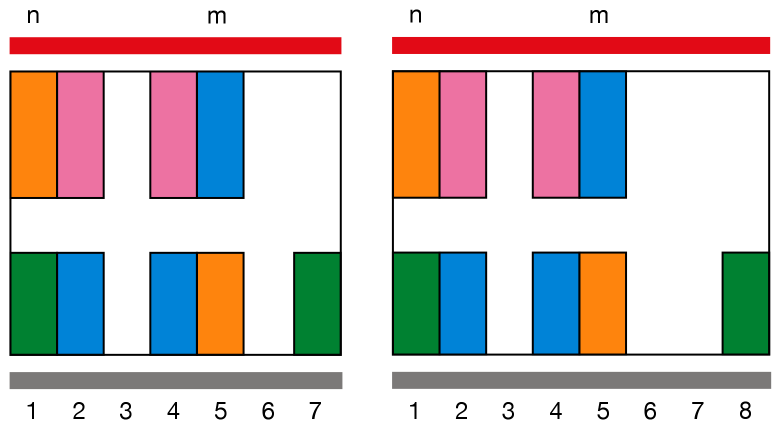
\includegraphics[scale=0.5]{img/design/pads.png}
  \caption{Partial problem with $pad = 1$ and $pad = 2$}
  \label{fig:pads}
\end{figure} 

Independently of what the partial routing algorithm is, after the results of a partial routing are copied back to the cell, an additional optimization can be performed. It consists on eliminating any wire that is not part of a path between two terminals. These wire segments are normally added because of the design rules or as connections to pins. They potentially occupy a space that is needed for a global routing to be found, and maybe another configuration which also respects the design rules and the pin connectivity can be reached in another routing stage. It is important to note, however, that such action must only be performed if the wires that are eliminated will be added again in a posterior routing of the same area, so that the final routing is correct. \\

This section has introduced the two most important approaches to cell partitioning. Other methods, composed of any of these algorithms and other variations, have been used. One of them, which was used in scan routing, is described in the next section. \\


\section{Meta-algorithms for Cell Routing}
\label{sec:metaalgorithms}

Given a complete cell we want to route, meta-algorithms define how to use partition algorithms, either the ones described before, variations or completely different ones, in order to find a solution which is valid for the whole cell. Most CellDivider versions use a bottom-up approach consisting on routing parts of the cell and finally trying to route the entire cell with the information provided by the partial solutions. However, other approaches were a final global routing is not needed have also been explored.  \\

It is important to remark that the number of possible meta-algorithms is enormous. Not only can they differ in the partitioning algorithms they use, but also in where and when they use them. The described meta-algorithms should be regarded as a methodology for cell routing using partial solutions. In every partial solution to the problem, parameters such as the halo have to be chosen. Any wrong decision could lead to an unsatisfiable solution and, given the case, how the meta-algorithm reacts is also of great relevance. \\



\subsection{2-Cell Routing}

This meta-algorithm was the first one used during the development of the project and is presented to illustrate the number of variables that can affect the execution of CellDivider. It consists on dividing the cell by the half and solving one or both parts to find a global solution. Now, which sides should be partially routed, the left one, the right one or both? Using realistic partitioning, boundary-conscious partitioning or a variation of any of them? What halo should be used when routing the partial problems? And when looking for a global routing? Even if this algorithm is very simple, this approach shows how big the experiment exploration can become. The number of parameters and decision combinations will only grow as the meta-algorithm's complexity increases. \\

However, 2-Cell routing is very limited. For example, when cells grow big, it can be interesting to divide the cell in more than two parts. This led to \textit{N-Cell Routing}, a variation of this algorithm in which the cell was divided in an arbitrary number of parts. For example, a cell such as the one in Figure \ref{fig:threebase} could be divided in three parts. A valid strategy would be to route the two side parts of the cell as shown in Figure \ref{fig:threemig}, which shows those parts already routed using boundary-conscious partitioning. Finally, we obtain the final problem and only routing it is left as seen on \ref{fig:threefinal}. Routing only the central part of the cell would also have been a valid approach. During development it was seen that partially routing the whole cell before doing the total routing would lead to unsatisfiability in many of the cases. However this method proves to be useful when the cell has a known physical structure such as concatenated cells. \\

\begin{figure}[h!]
  \centering
  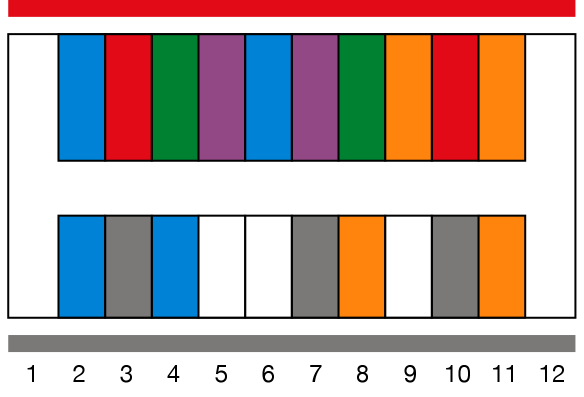
\includegraphics[scale=0.5]{img/design/threebase.png}
  \caption{Input for CellDivider}
  \label{fig:threebase}
\end{figure} 

\begin{figure}[h!]
  \centering
  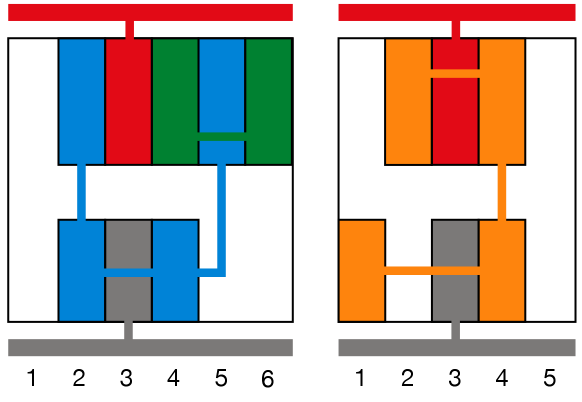
\includegraphics[scale=0.5]{img/design/threemig.png}
  \caption{Partial problems and solutions}
  \label{fig:threemig}
\end{figure} 

\begin{figure}[h!]
  \centering
  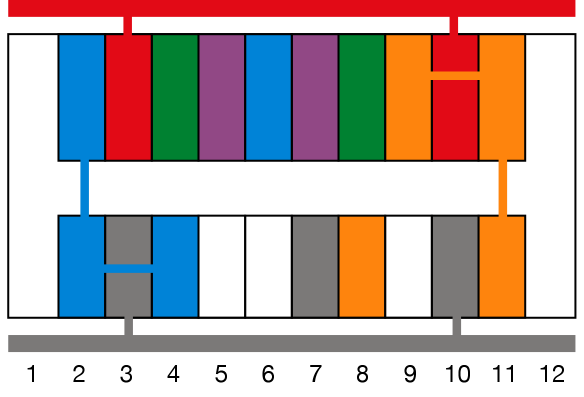
\includegraphics[scale=0.5]{img/design/threefinal.png}
  \caption{Final routing problem}
  \label{fig:threefinal}
\end{figure} 

After some experimentation, blindly partitioning the cell in equal chunks still seemed quite a basic approach. Additionally, this meta-algorithm needs for a total route of the entire cell as a last step. The meta-algorithms that will be described in the following subsections try to take such observations into account. Many variations of them are also possible but have not been explored. \\

\subsection{Congestion-Driven Routing}

When deciding which part of the cell to route before, first solving the most congested part seemed a good approach. Given that we want to avoid a final unsatisfiable result, the idea is dealing with the hard parts in the first instance so that later only easy to route parts are left. \\

The idea to measure congestion is simple: The number of subnets that must cross each column. This can be calculated easily by scanning the cell from side to side and considering the first and last appearance of each signal. Each one of them will add congestion to every column between the first and the last appearance. A wire of said signal will have to cross each one of these columns in order to connect all the terminals of the net. Figure \ref{fig:congestion} shows a cell with the congestion vale of each column above it. \\

\begin{figure}[h!]
  \centering
  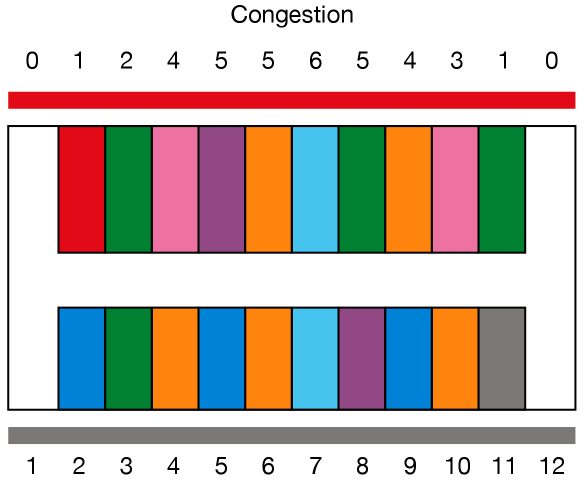
\includegraphics[scale=0.5]{img/design/congestion.png}
  \caption{Congestion of the columns in a cell}
  \label{fig:congestion}
\end{figure} 

Congestion-driven routing can be applied in a wide range of ways. Here follow some of the versions that were developed. \\

\begin{description}
  \item[Window Routing] \hfill \\
  	This method uses a window of a fixed length $w$, which is either a number given with the input or some measure relative to the width (for example, a half or a third of its width). It proceeds by partially routing the zone of the cell with width $w$ such that the sum of the congestion of the columns in the zone is maximal. It usually falls somewhere in the middle of the cell, which usually is the most congested part. Figure \ref{fig:congestionwindow} shows what part of the cell would be partially routed in the one presented above. The implementation was abandoned to try other strategies and did not allow for multiple overlapping partial routings at the time. The pseudocode is as follows. \\
  	

\small
\begin{algorithmic}
\Function{Window routing}{$G$ grid, $w$ window size} \\
\State $time \gets 0$
\State $histogram \gets histogram(G)$
\State $zone \gets congested_zone(histogram, w)$ \\

\State $partial\_route \gets route\_range(G, range)$
\If {$partial\_route.state = SAT$}
	\State $time \gets time + partial\_route.time$
\Else
	\State \Return $unsat$
\EndIf \\

\State $total\_route \gets route(G)$
\If {$total\_route.state = SAT$}
	\State \Return $time + total\_route.time$
\Else
	\State \Return $unsat$
\EndIf

\EndFunction
\end{algorithmic}
\normalsize
  	
  \item[Zone Routing] \hfill \\
    This method used the congestion metric in a different way. It incorporated a function that, given the congestion value of each column, returned a set of column ranges that should be partially routed. The one used considered those zones were congestion was maximum and only on unit under the maximum, but different strategies can be applied. Those zones have a variable length which can vary for different zones in the same execution. From the cells used during experimentation, the partially routed area amounted from a 14\% to a 95\% of the cell. For example, if applied to the cell introduced in this subsection on Figure \ref{fig:congestion}, the zone that would be routed is between the $5$th and $8$th columns as shown in Figure \ref{fig:congestionzone}, but on bigger cells it would produce several partial routings. This would be a version in pseudocode. \\
    
\small
\begin{algorithmic}
\Function{Zone routing}{$G$ grid} \\
\State $time \gets 0$
\State $histogram \gets histogram(G)$
\State $zones \gets congested_zones(histogram)$ \\

\ForAll{$zone$ in $zones$} 
	\State $partial\_route \gets route\_range(G, zone.begin, zone.end)$
	\If {$partial\_route.state = SAT$}
		\State $time \gets time + partial\_route.time$
	\Else
		\State \Return $unsat$
	\EndIf
\EndFor

\State $total\_route \gets route(G)$
\If {$total\_route.state = SAT$}
	\State \Return $time + total\_route.time$
\Else
	\State \Return $unsat$
\EndIf

\EndFunction
\end{algorithmic}    
\normalsize
\end{description}


\begin{figure}[h!]
  \centering
  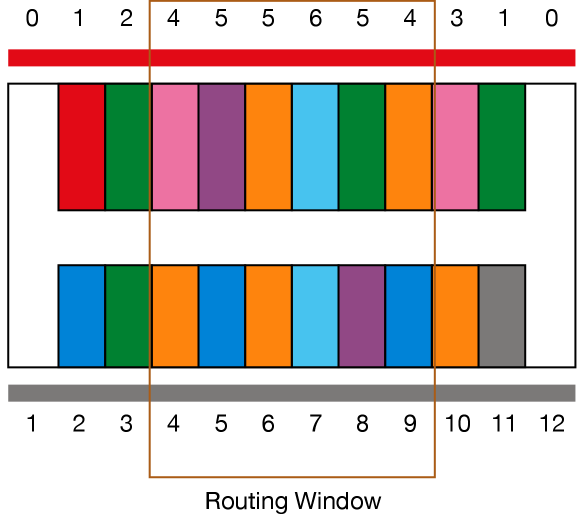
\includegraphics[scale=0.5]{img/design/congestionwindow.png}
  \caption{Window routing example}
  \label{fig:congestionwindow}
\end{figure} 

\begin{figure}[h!]
  \centering
  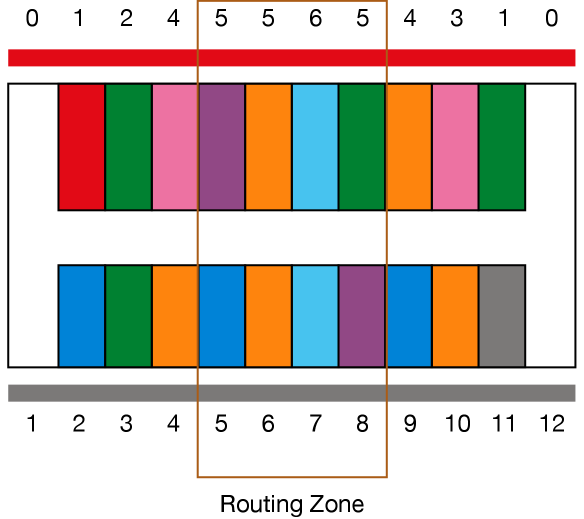
\includegraphics[scale=0.5]{img/design/congestionzone.png}
  \caption{Zone routing example}
  \label{fig:congestionzone}
\end{figure} 

No more work was done in congestion-driven routing when development of the last meta-algorithm began. All of these methods require of a final routing step where the whole cell is included, which was something that we wanted to avoid as will be seen in next sub-section. \\



\subsection{Scan Routing}

The aim of scan routing is to route the cell without the need of a final step where the whole cell is codified into a SAT formula. In order to do so, the cell is divided in a given number of contiguous chunks which are then routed from left to right. After routing the $i$th part of the cell, all subnets which should both begin and end in the $i$th chunk or before are already routed. This way, after routing the final division of the cell, the whole cell has been routed. In order to do so, considering we want to route from column $n$ to column $m$, the partitioning algorithm used is as follows. \\

For the part at the left of this zone we use the approach of the realistic partition algorithm with the variant where all the terminals and wires of the already routed zone are included on the partial problem. In scan routing, we consider that the left part of a partial routing has already been routed and incorporated to the final solution. If this is not regarded when routing the next part, it is possible that the new partial solution would need to assign certain signals to positions were a different wire has already been defined. The boundary-conscious partitioning approach can not be used in this part, given that it does not respect the geometry of the cell and does easily lead to unsatisfiable solutions. When obtaining a partial result, all wires at the left of $n$ will be considered as fixed and all wires at the right of $m$ will be discarded, given that we only wanted to impose that a path from the zone we already routed and some signals at the right of column $m$ existed. Additionally, some cleaning of not necessary wires in the left part is performed before a partial routing, knowing that the router will put them back again if they are really necessary. \\

On the right part of the zone we want to route we will use the approximation routing approach. This way we can potentially save a lot of blank space when looking for the partial solution. It is not so important to keep the original geometry, given that the part in the right will not be fixed after the partial routing. \\

The partial solutions used in scan routing, thus, take advantage of both of the approaches introduced in Section \ref{sec:partitionalgorithms}. After all the parts of the cell have been routed from left to right, a solution for the routing of the whole cell is obtained. Signals that need to have a connection pin only require it on the first partial routing where they appear, given that from then on all the other terminals of the net will be connected to the subnets of the first part, which are connected to the pin. Partial routings are optimized in order to raise the chances of getting a satisfying assignment and, at the same time, yield better final solutions. However, as happens with the other methods, scan routing not finding a solution does not imply it does not exist. The pseudocode looks as follows.\\

\small
\begin{algorithmic}
\Function{Scan routing}{$G$ grid, $n$ number of parts} \\
\State $time \gets 0$
\State $ranges \gets $ boundaries of the $n$ parts of $G$
\ForAll{$range$ in $ranges$ ordered from left to right} 
	\State $partial\_route \gets route\_range(G, range)$
	\If {$partial\_route.state = SAT$}
		\State $time \gets time + partial\_route.time$
	\Else
		\State \Return $unsat$
	\EndIf
\EndFor
\EndFunction

\end{algorithmic} 
\normalsize


The following example will illustrate how the algorithm works. Consider the cell in Figure \ref{fig:scanbase}. \\

\begin{figure}[h!]
  \centering
  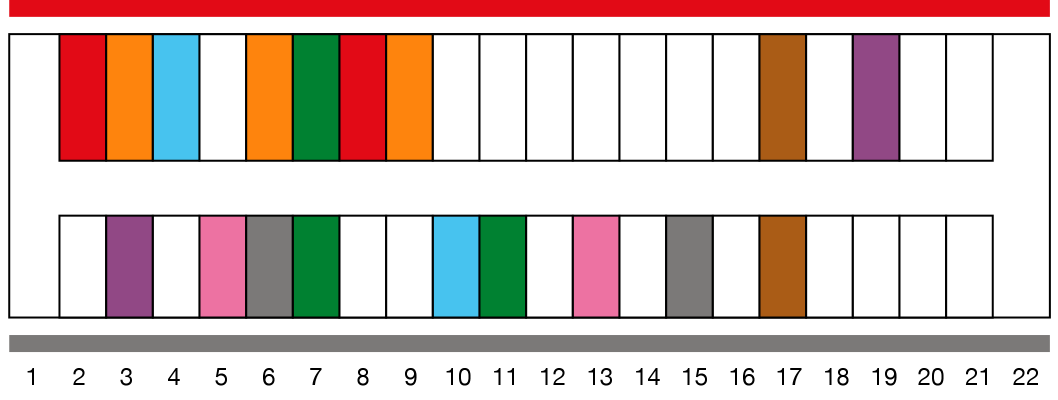
\includegraphics[scale=0.5]{img/design/scanbase.png}
  \caption{Input for CellDivider}
  \label{fig:scanbase}
\end{figure} 
\vspace{10 mm}
We decide to use the scan algorithm on that cell in three parts. The cell is divided into the following ranges: $(1, 8)$, $(9, 15)$ and $(16, 22)$. Figure \ref{fig:scanpart1} shows the routing of the first part. In this case, the closest terminal of all signals which are to be connected to a net in the $(1, 8)$ range are approximated to the boundary. Figure \ref{fig:scantotal1} shows the state of the whole cell after the partial routing has been added. \\

\begin{figure}[h!]
  \centering
  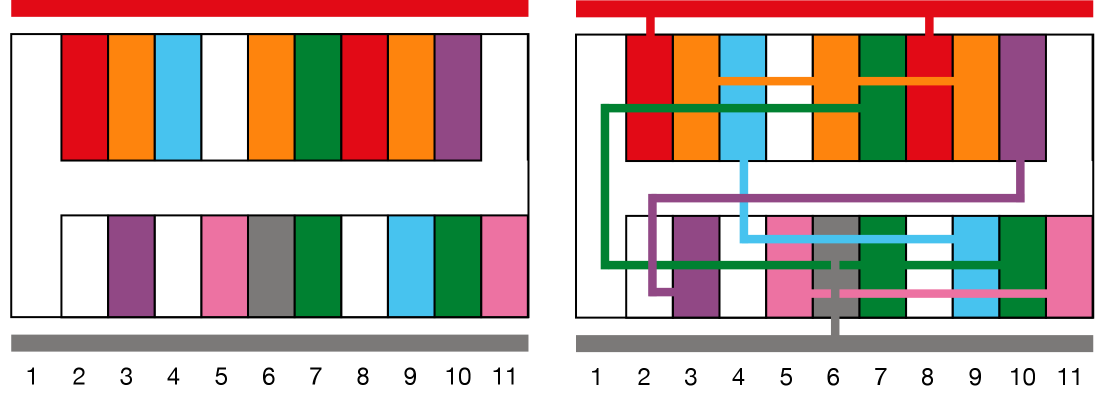
\includegraphics[scale=0.5]{img/design/scanpart1.png}
  \caption{Partial routing, first part}
  \label{fig:scanpart1}
\end{figure} 

\begin{figure}[h!]
  \centering
  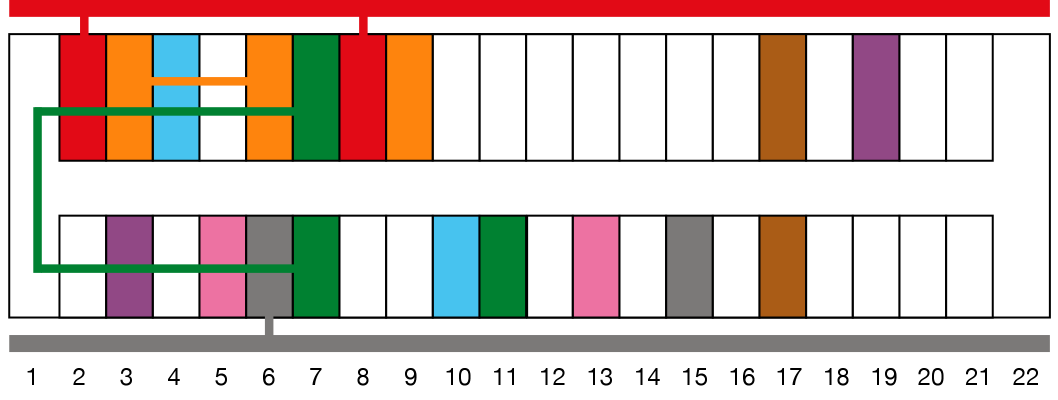
\includegraphics[scale=0.5]{img/design/scantotal1.png}
  \caption{Cell after first partial routing}
  \label{fig:scantotal1}
\end{figure} 

Now it is time to route the second range as seen in Figure \ref{fig:scanpart2}. This time only one signal will be come closer on the right side. However, a big part of the already routed cell will be included in the partial routing, as some of the terminals in $(9, 15)$ have to be routed with terminals in the already routed part. Figure \ref{fig:scantotal2} shows the state of the cell after this second routing. \\

\begin{figure}[h!]
  \centering
  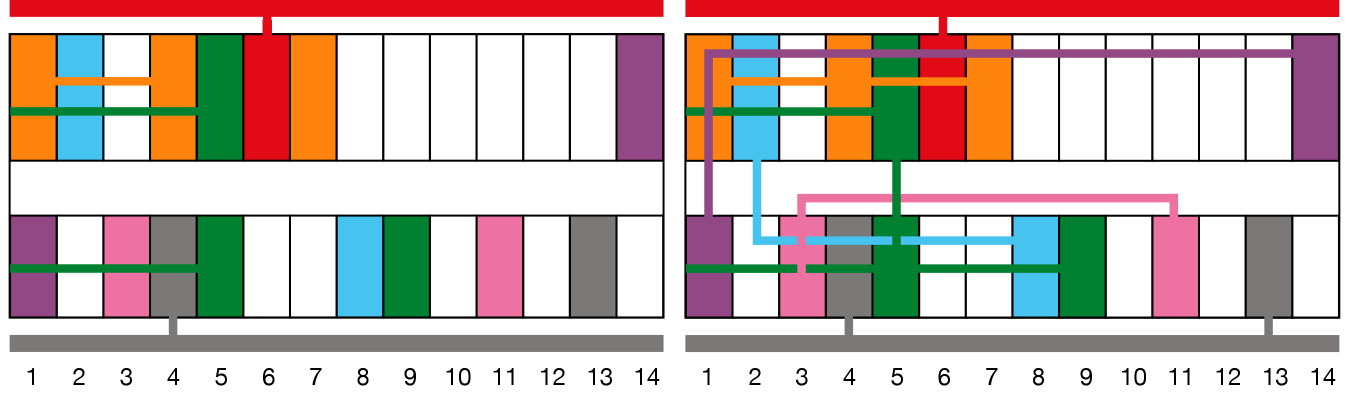
\includegraphics[scale=0.5]{img/design/scanpart2.png}
  \caption{Partial routing, second part}
  \label{fig:scanpart2}
\end{figure} 

\begin{figure}[h!]
  \centering
  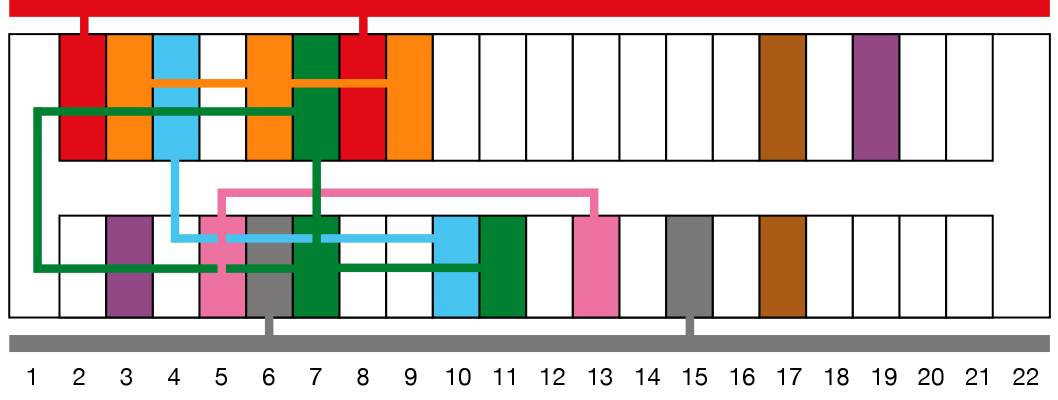
\includegraphics[scale=0.5]{img/design/scantotal2.png}
  \caption{Cell after second partial routing}
  \label{fig:scantotal2}
\end{figure} 

The last step is to route the third part of the cell. After the last partial solution is computed, no more routing is be needed. Figure \ref{fig:scantotal3} shows the solution for the last partial routing and how it is all integrated in the cell. \\

\begin{figure}[h!]
  \centering
  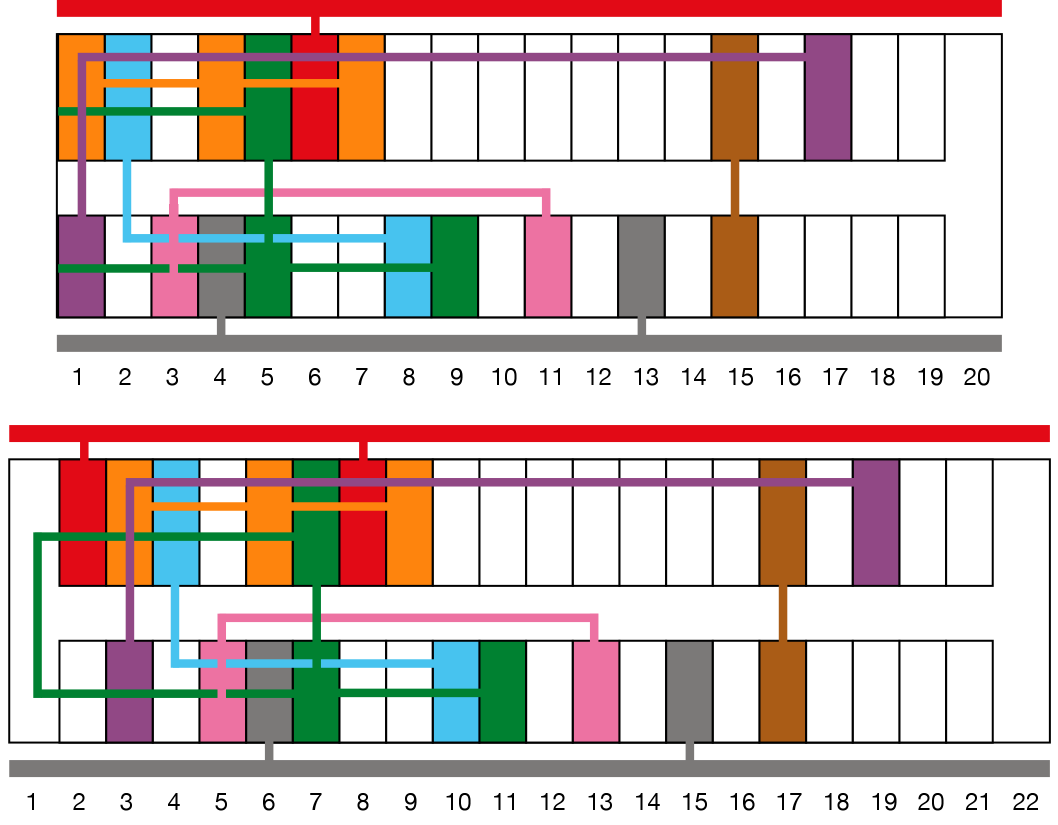
\includegraphics[scale=0.5]{img/design/scantotal3.png}
  \caption{Third partial routing and final solution}
  \label{fig:scantotal3}
\end{figure} 


However, the scan algorithm needs an extra tweaking on the partitioning algorithm. Notice how the terminals on column 6 have been routed twice. This is because when doing the second partial routing, as seen in Figure \ref{fig:scanpart2}, the connection of those terminals disappeared beyond the left boundary. The following addition is included to solve this problem. When the left border is known, the algorithm checks if in that column more than one wire for the same signal exists and, if they are not connected, the shortest path between those positions is added to the partial problem. Given that this implies expanding the cell by the left side, all positions that are not part of a shortest path are blocked. Figure \ref{fig:scanalt} shows how the second partial routing problem is. The black zone represents positions that can not be modified but have been added in order to let the router know that both terminals on the original column 6 are already connected. Avoiding duplicate connections is important since they could mean the difference between a satisfiable and an unsatisfiable cell. \\

\begin{figure}[h!]
  \centering
  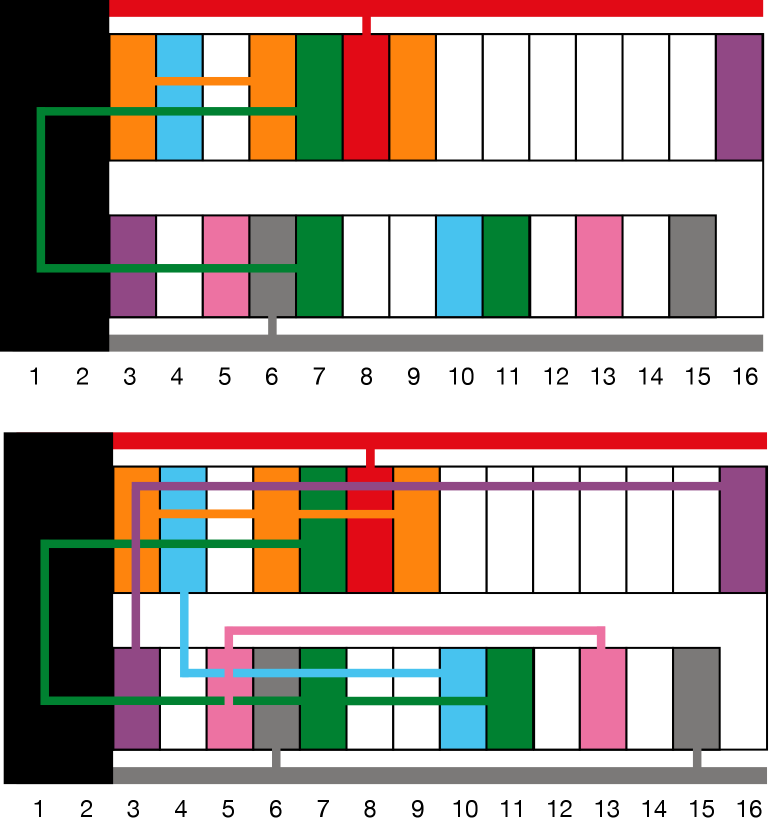
\includegraphics[scale=0.5]{img/design/scanalt.png}
  \caption{Second partial routing with blocks and solution}
  \label{fig:scanalt}
\end{figure} 

As we wanted, the scan approach has an important benefit over the others: it does not need a total routing over the cell. This is very interesting because, when cells get big and the number of signals increases, the generation of the formula can become expensive. Besides, never having the whole formula at once allows to route cells using less maximum RAM memory. However, this method also turns out to produce many unsatisfiable cells, specially when they are very congested. \\


\section{Conclusions}

This chapter has presented the algorithms that have been used to both route a part of a cell and to use these partial routing to obtain a global valid solution. Many more options and variants could have been explored but these seemed the ones that could lead to a better final solution. The following section focuses on the results of several experiments done using most of the algorithms that have been introduced in this section on several kinds of cells.